\section{Giao diện Website và Bảng điều khiển}

Giao diện trạm học tập Pomodoro được xây dựng trên nền tảng Node-RED Dashboard hiện đại, cung cấp khả năng hiển thị đáp ứng (responsive) trên cả máy tính để bàn (Desktop) và điện thoại thông minh (Mobile). Hệ thống cho phép người học dễ dàng theo dõi môi trường bàn học, kiểm soát tiến độ Pomodoro và gửi lệnh tương tác trực tiếp tới phần cứng.

\subsection{Nhận xét giao diện và mức độ phức tạp}
Giao diện quản lý được tổ chức thành các phân vùng chức năng mạch lạc:
\begin{itemize}
    \item \textbf{Phân hệ xác thực (Auth):} Bảo vệ hệ thống bằng màn hình đăng ký và đăng nhập bảo mật trước khi truy cập dữ liệu cá nhân.
    \item \textbf{Bàn làm việc chính (Workspace):} Tích hợp các widget thời gian thực gồm đếm ngược Pomodoro, form gửi chữ lên LCD, các đồng hồ đo vi khí hậu (DHT22, quang trở) và nhật ký hoạt động gần nhất.
    \item \textbf{Lịch sử và Thống kê (History):} Trực quan hóa dữ liệu lịch sử các phiên học và chuỗi biến thiên môi trường dưới dạng biểu đồ đường và biểu đồ cột.
    \item \textbf{Cài đặt hệ thống (Settings):} Cung cấp các thanh trượt cấu hình ngưỡng nhiệt độ, thời gian cảnh báo và thông tin kết nối Telegram, Gmail.
\end{itemize}

Về mức độ phức tạp, website không chỉ dừng lại ở các chức năng hiển thị CRUD cơ bản mà còn đòi hỏi xử lý truyền thông hai chiều thời gian thực qua giao thức MQTT/WebSocket, tích hợp xác thực mật khẩu bcrypt, truy vấn dữ liệu chuỗi thời gian trên Supabase và tự động đồng bộ hóa trạng thái hai chiều giữa phần cứng ESP32 và màn hình điều khiển.

\subsection{Màn hình Đăng nhập hệ thống}
Giao diện đăng nhập đảm bảo an toàn thông tin cá nhân. Người dùng cần nhập đúng thông tin tài khoản đã đăng ký trên Supabase để mở khóa các tính năng quản trị và điều khiển.

\begin{figure}[htbp]
\centering
\begin{subfigure}[b]{0.62\textwidth}
    \centering
    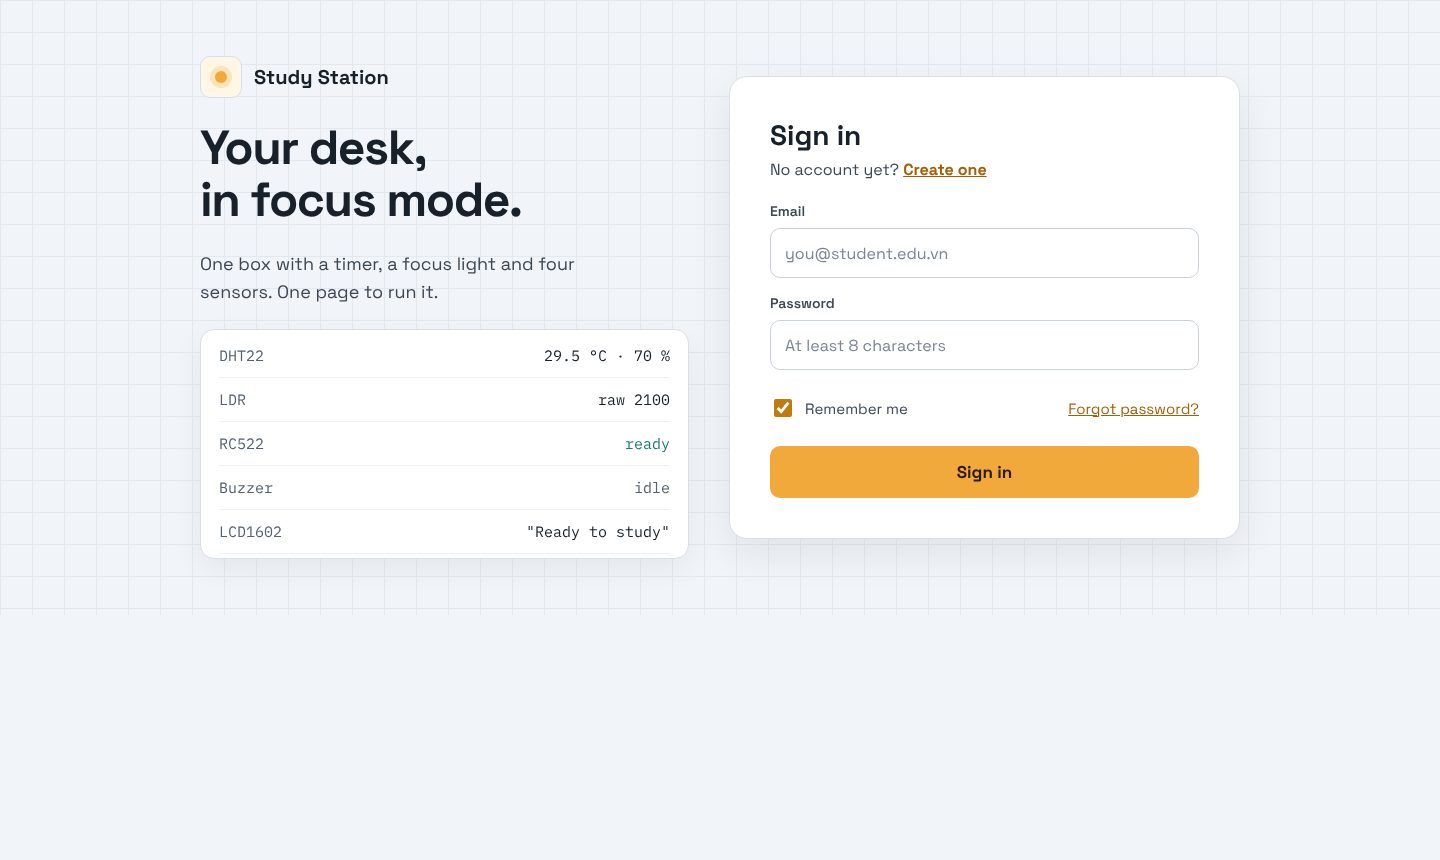
\includegraphics[width=\textwidth]{assets/wireframes/01-sign-in-desktop.png}
    \caption{Giao diện Đăng nhập trên Desktop}
    \label{fig:signin_desktop}
\end{subfigure}
\hfill
\begin{subfigure}[b]{0.32\textwidth}
    \centering
    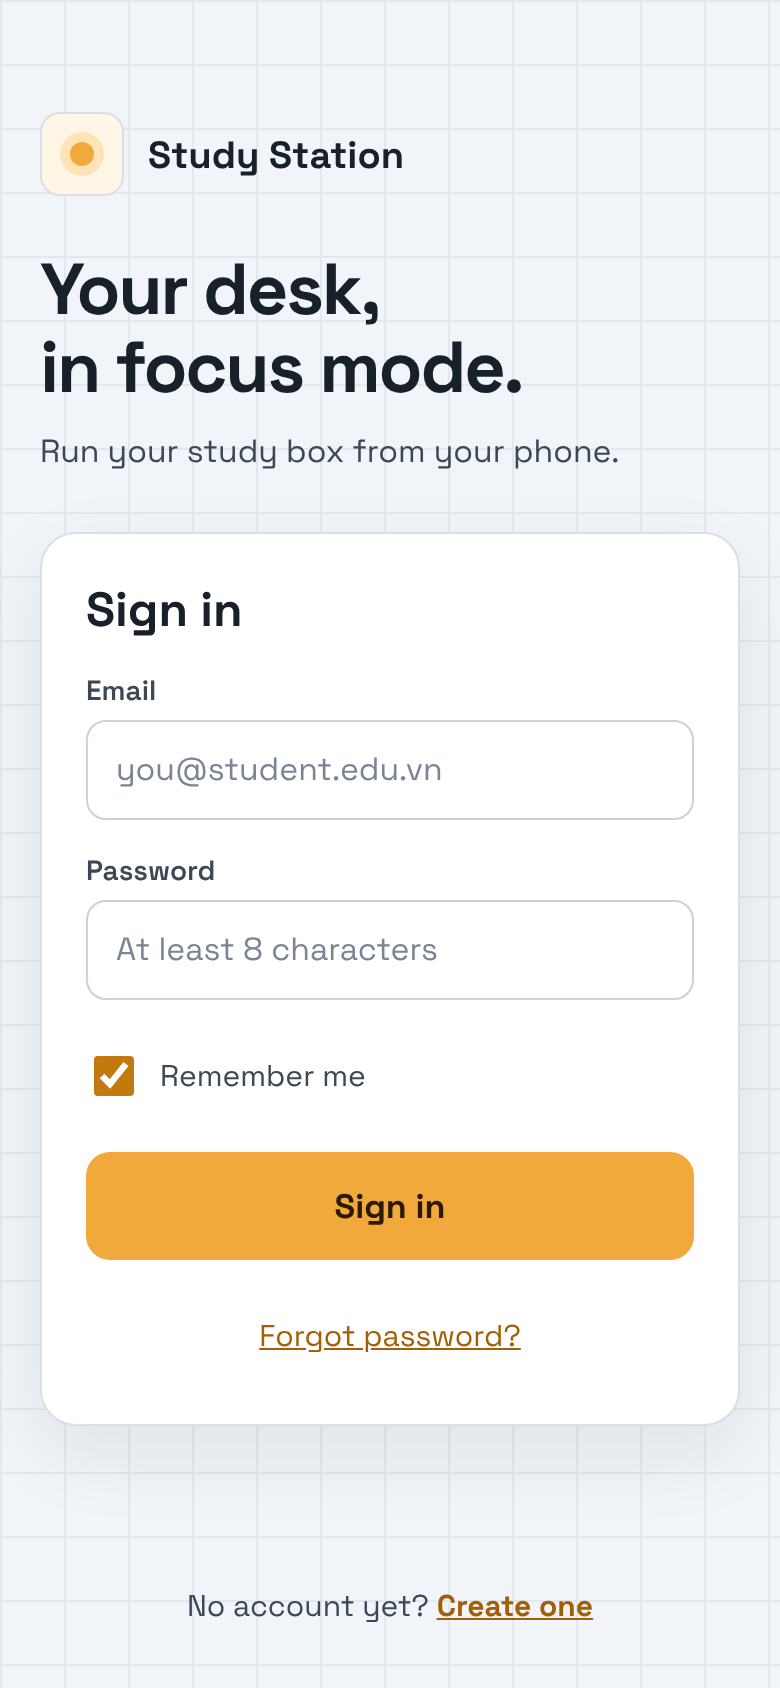
\includegraphics[width=\textwidth]{assets/wireframes/05-sign-in-mobile.png}
    \caption{Giao diện trên Mobile}
    \label{fig:signin_mobile}
\end{subfigure}
\caption{Giao diện Đăng nhập hệ thống trên nền tảng Desktop và Mobile}
\label{fig:sign_in}
\end{figure}

\subsection{Bàn làm việc chính (Workspace)}
Màn hình Workspace là trung tâm điều khiển phiên học. Tại đây, người dùng có thể kích hoạt hẹn giờ, xem nhiệt độ, độ ẩm, trạng thái ánh sáng và gửi nội dung lời nhắc lên màn hình LCD.

\begin{figure}[htbp]
\centering
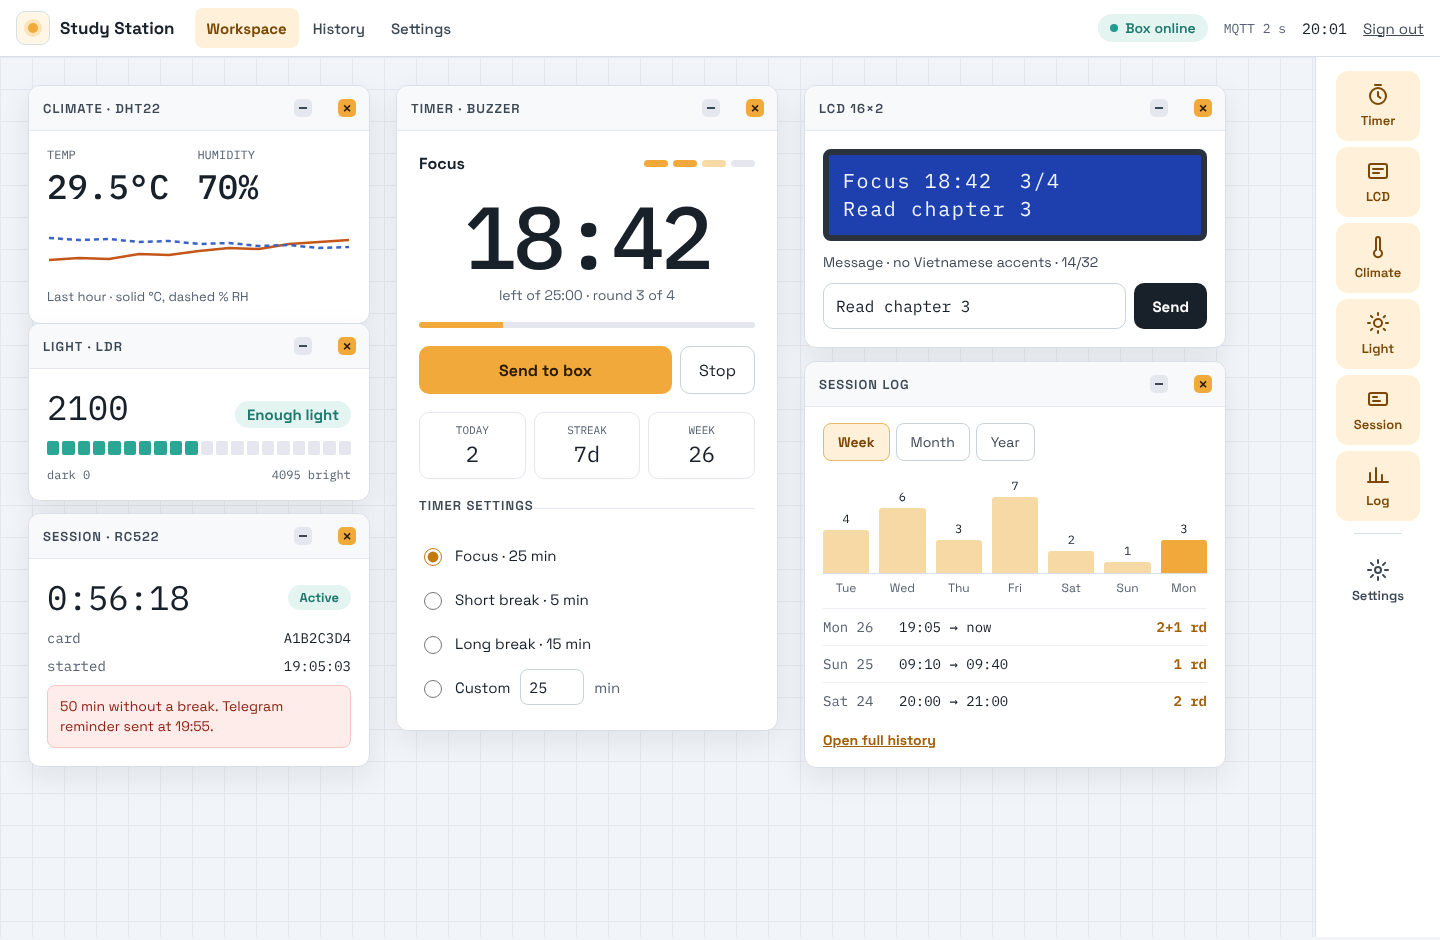
\includegraphics[width=0.92\textwidth]{assets/wireframes/02-workspace-desktop.png}
\caption{Giao diện Bàn làm việc tổng quan (Workspace) trên Desktop}
\label{fig:workspace_desktop}
\end{figure}

\subsection{Các khối chức năng chi tiết trên giao diện di động}

Để đảm bảo tính linh hoạt khi sử dụng điện thoại tại bàn học, giao diện Workspace được tối ưu hóa theo dạng các thẻ module độc lập:

\begin{figure}[htbp]
\centering
\begin{subfigure}[b]{0.46\textwidth}
    \centering
    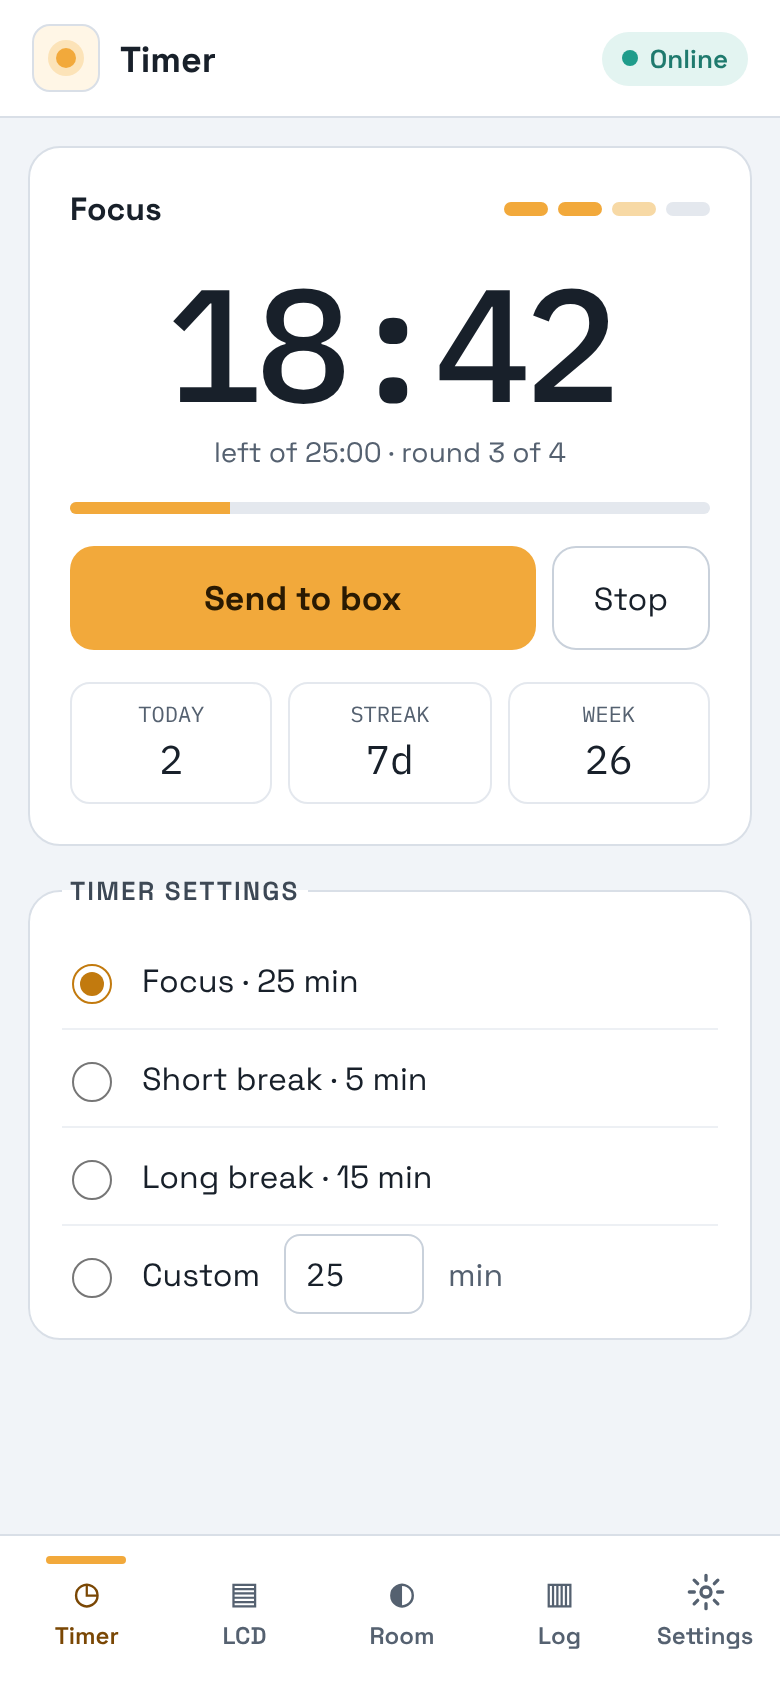
\includegraphics[width=\textwidth]{assets/wireframes/06-workspace-mobile-timer.png}
    \caption{Khối điều khiển hẹn giờ Pomodoro}
    \label{fig:mobile_timer}
\end{subfigure}
\hfill
\begin{subfigure}[b]{0.46\textwidth}
    \centering
    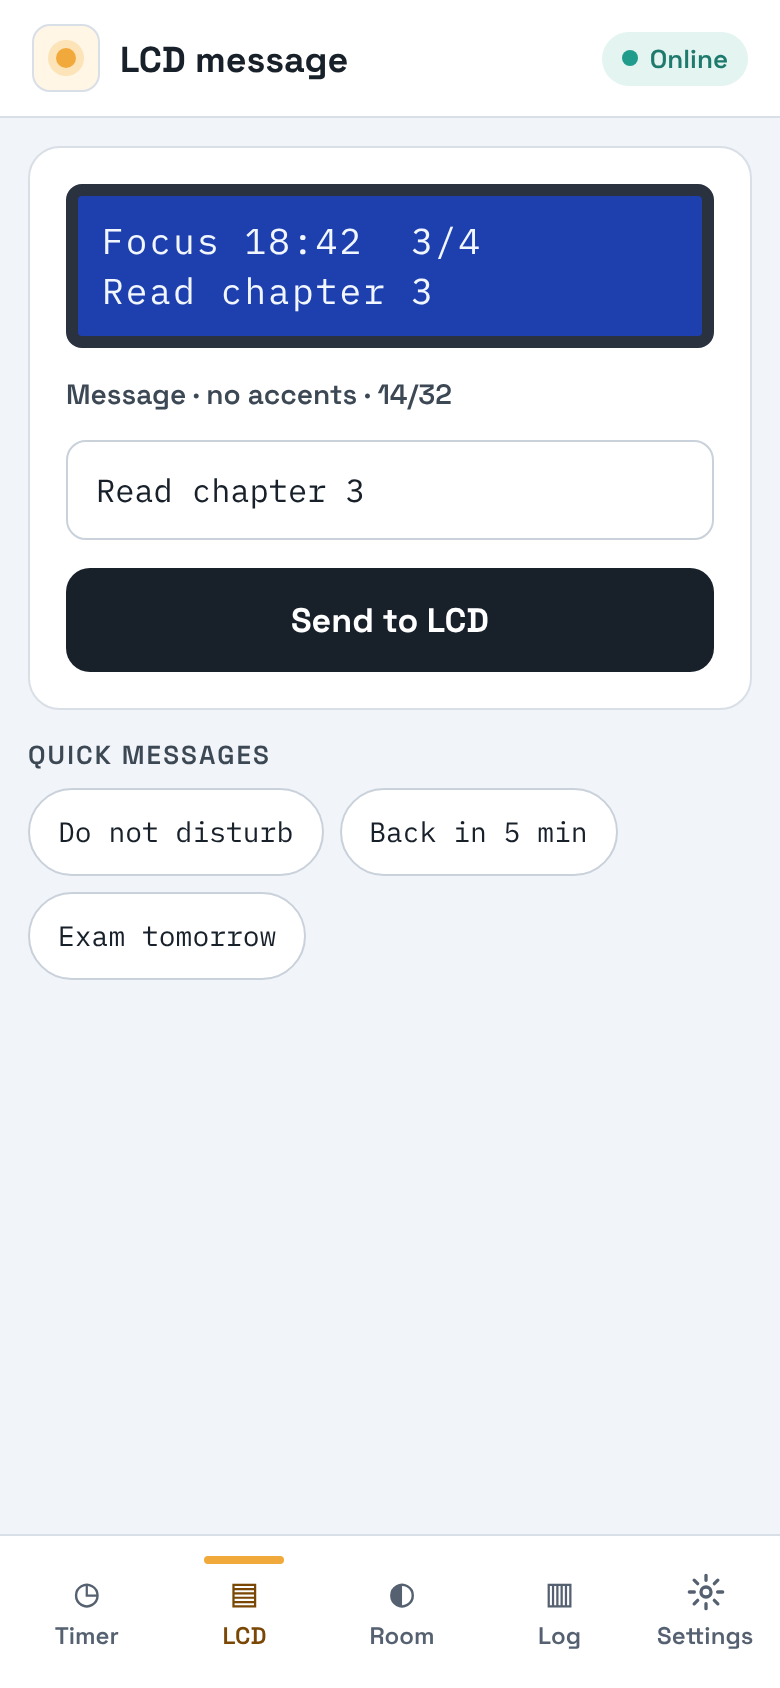
\includegraphics[width=\textwidth]{assets/wireframes/07-workspace-mobile-lcd.png}
    \caption{Khối gửi lời nhắc văn bản lên LCD}
    \label{fig:mobile_lcd}
\end{subfigure}
\caption{Các phân vùng điều khiển phiên học trên giao diện Mobile}
\label{fig:workspace_mobile_controls}
\end{figure}

\begin{figure}[htbp]
\centering
\begin{subfigure}[b]{0.46\textwidth}
    \centering
    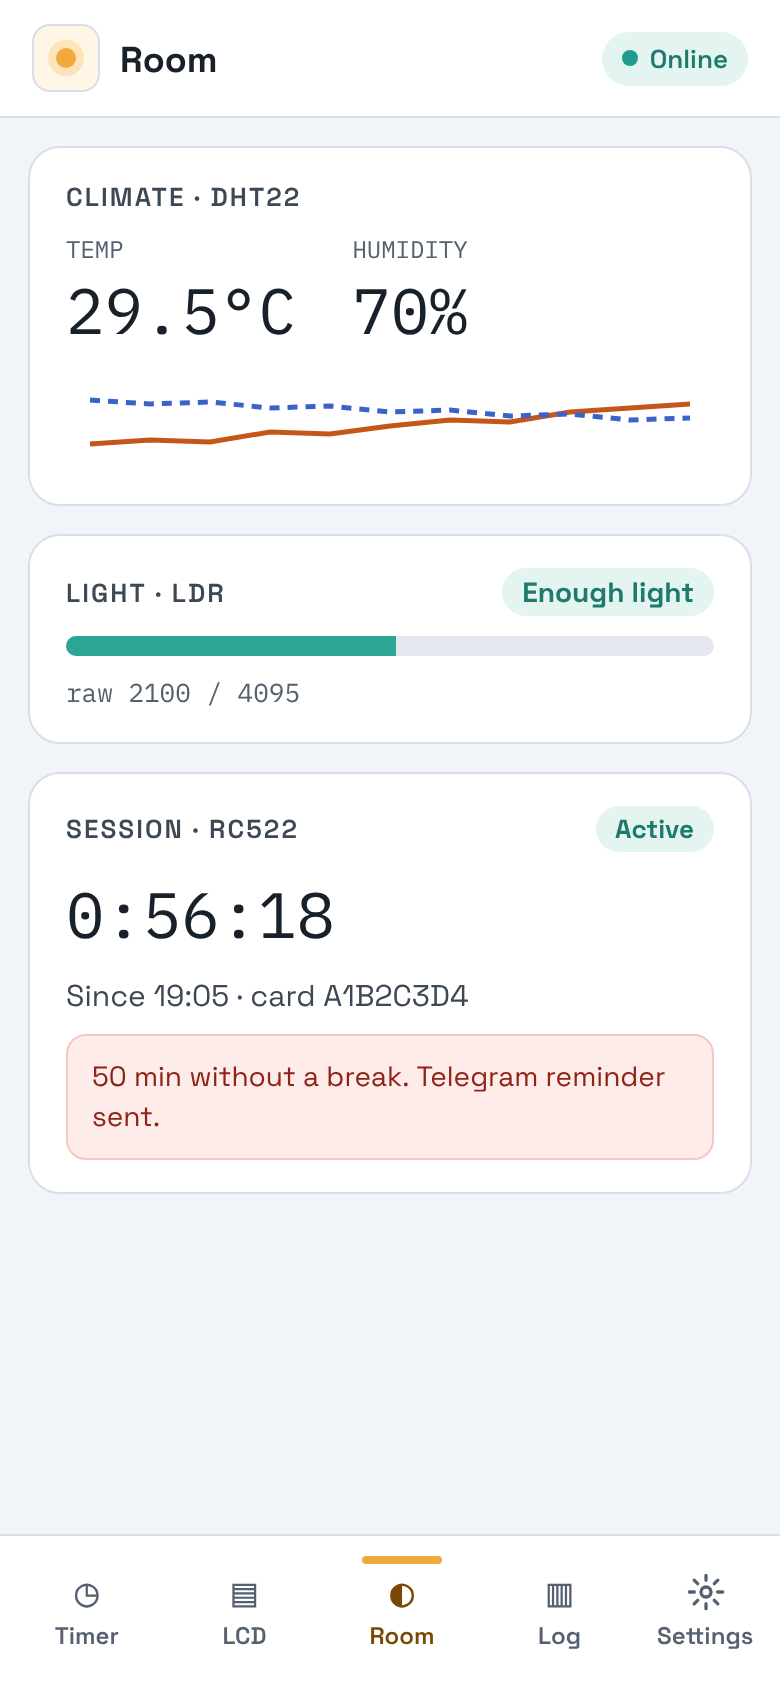
\includegraphics[width=\textwidth]{assets/wireframes/08-workspace-mobile-room.png}
    \caption{Khối giám sát nhiệt độ, độ ẩm \& ánh sáng}
    \label{fig:mobile_room}
\end{subfigure}
\hfill
\begin{subfigure}[b]{0.46\textwidth}
    \centering
    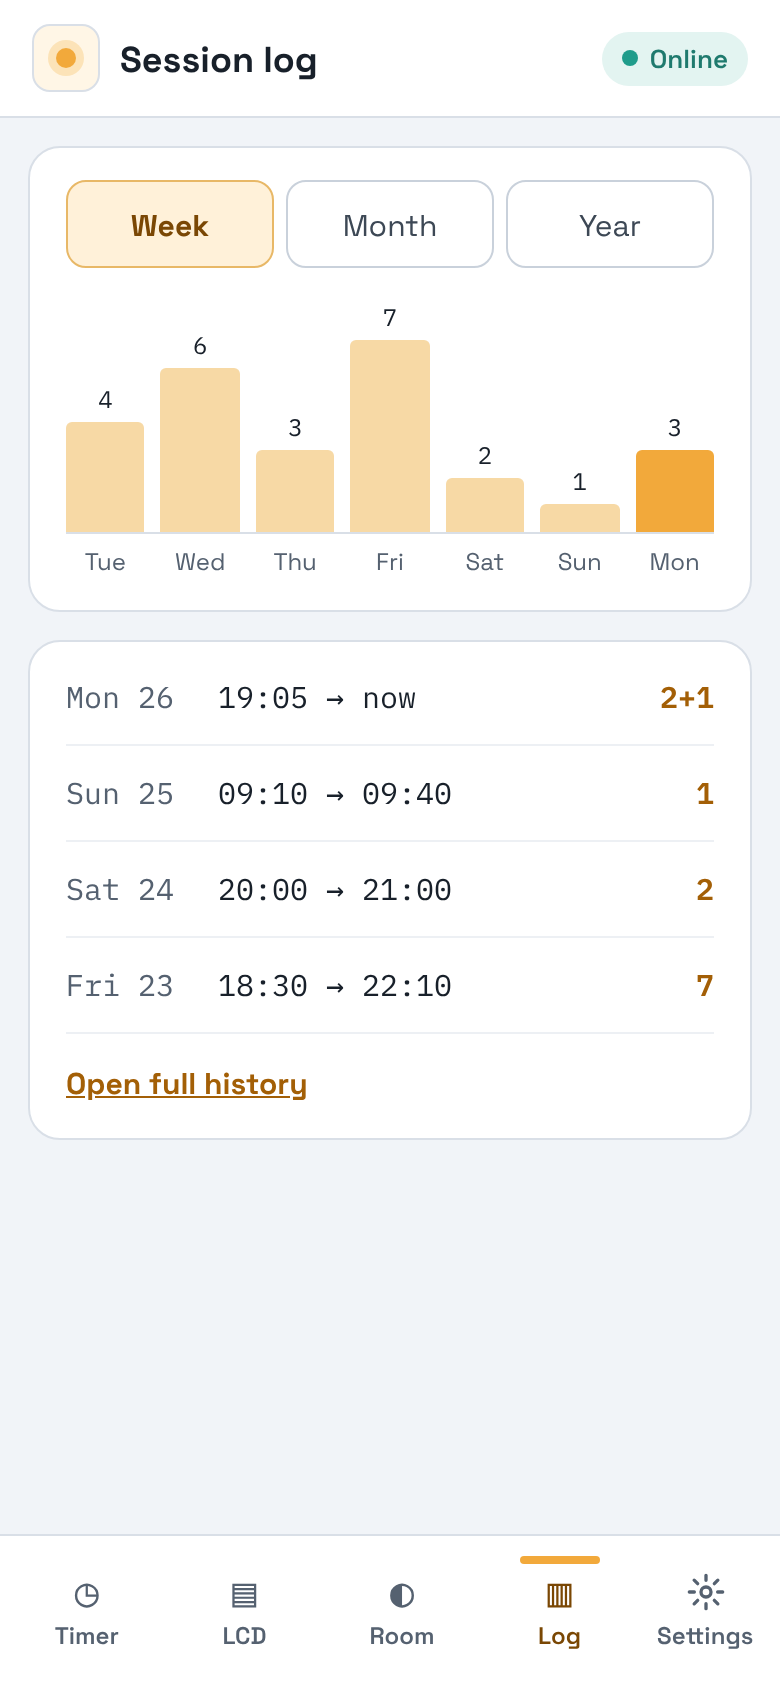
\includegraphics[width=\textwidth]{assets/wireframes/09-workspace-mobile-log.png}
    \caption{Khối nhật ký sự kiện thời gian thực}
    \label{fig:mobile_log}
\end{subfigure}
\caption{Các phân vùng giám sát môi trường và nhật ký trên giao diện Mobile}
\label{fig:workspace_mobile_monitoring}
\end{figure}

\subsection{Màn hình Lịch sử và Thống kê}
Trang Lịch sử cung cấp cái nhìn trực quan về kỷ luật học tập thông qua biểu đồ biến thiên các thông số môi trường theo giờ và tổng số phiên Pomodoro hoàn thành mỗi ngày trong tuần.

\begin{figure}[htbp]
\centering
\begin{subfigure}[b]{0.62\textwidth}
    \centering
    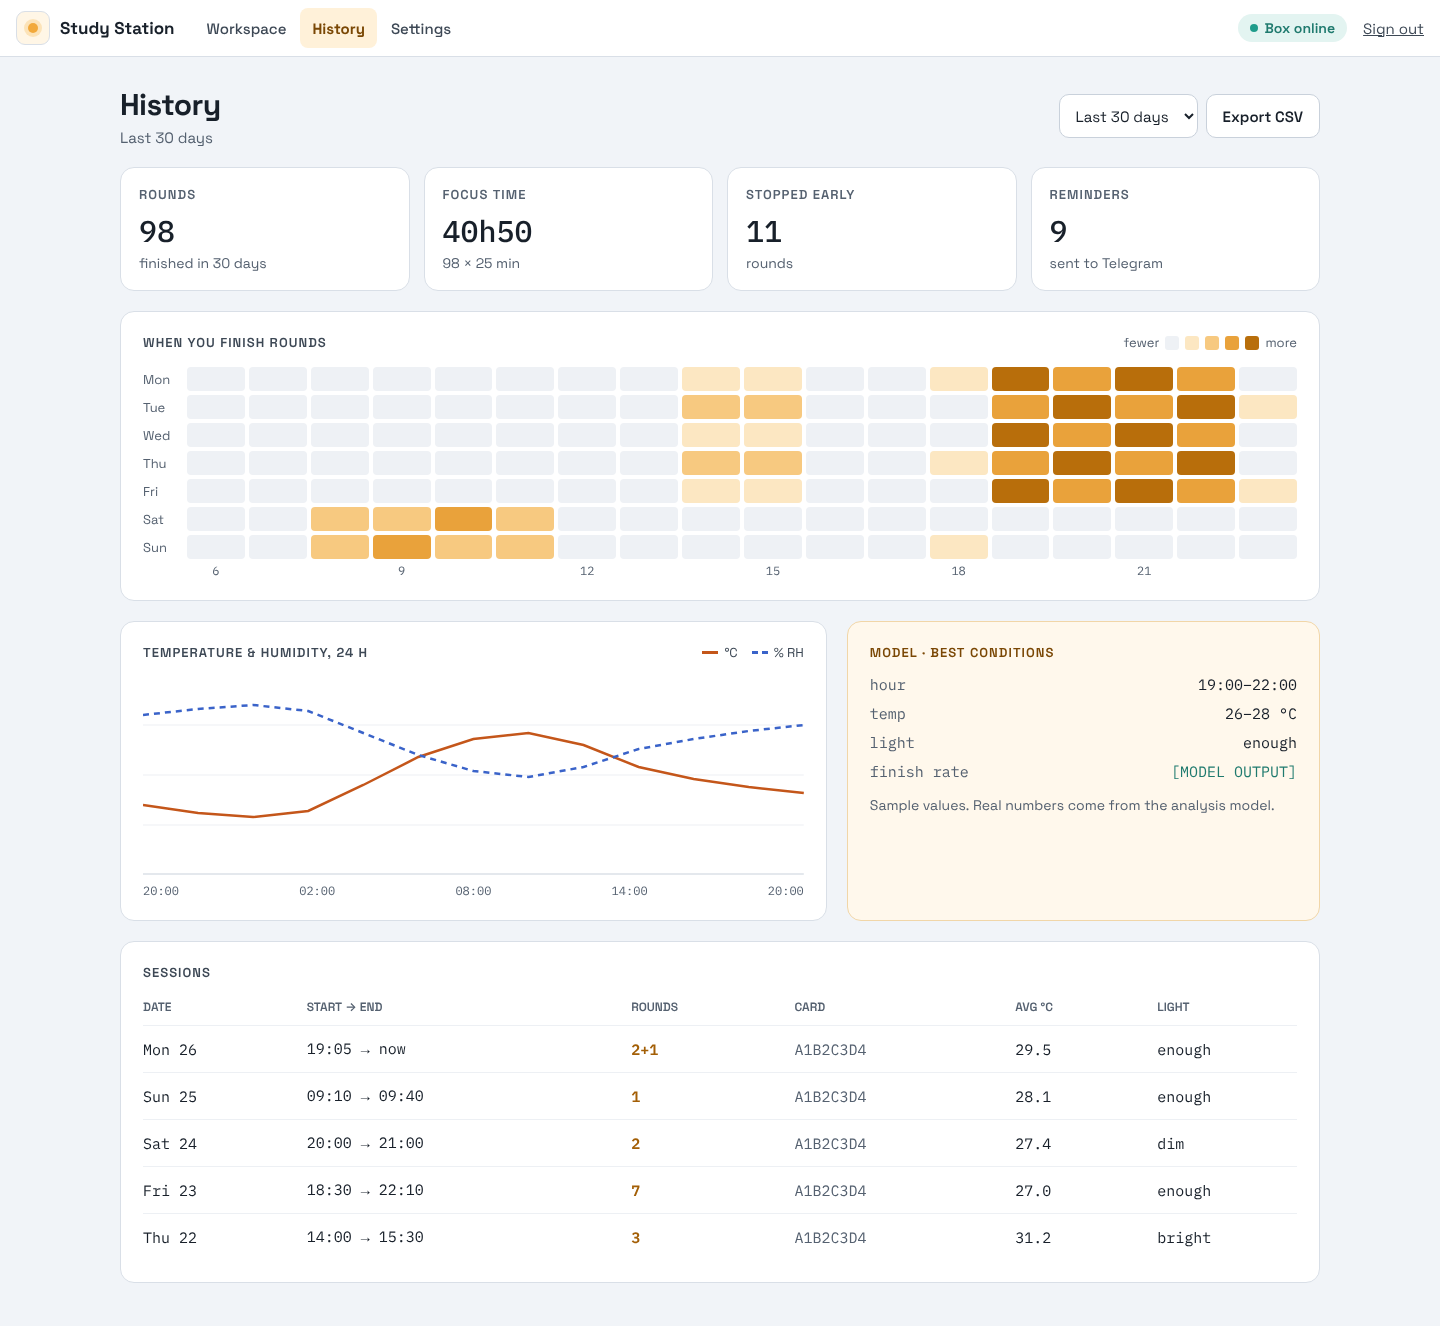
\includegraphics[width=\textwidth]{assets/wireframes/03-history-desktop.png}
    \caption{Trang Lịch sử trên Desktop}
    \label{fig:history_desktop}
\end{subfigure}
\hfill
\begin{subfigure}[b]{0.32\textwidth}
    \centering
    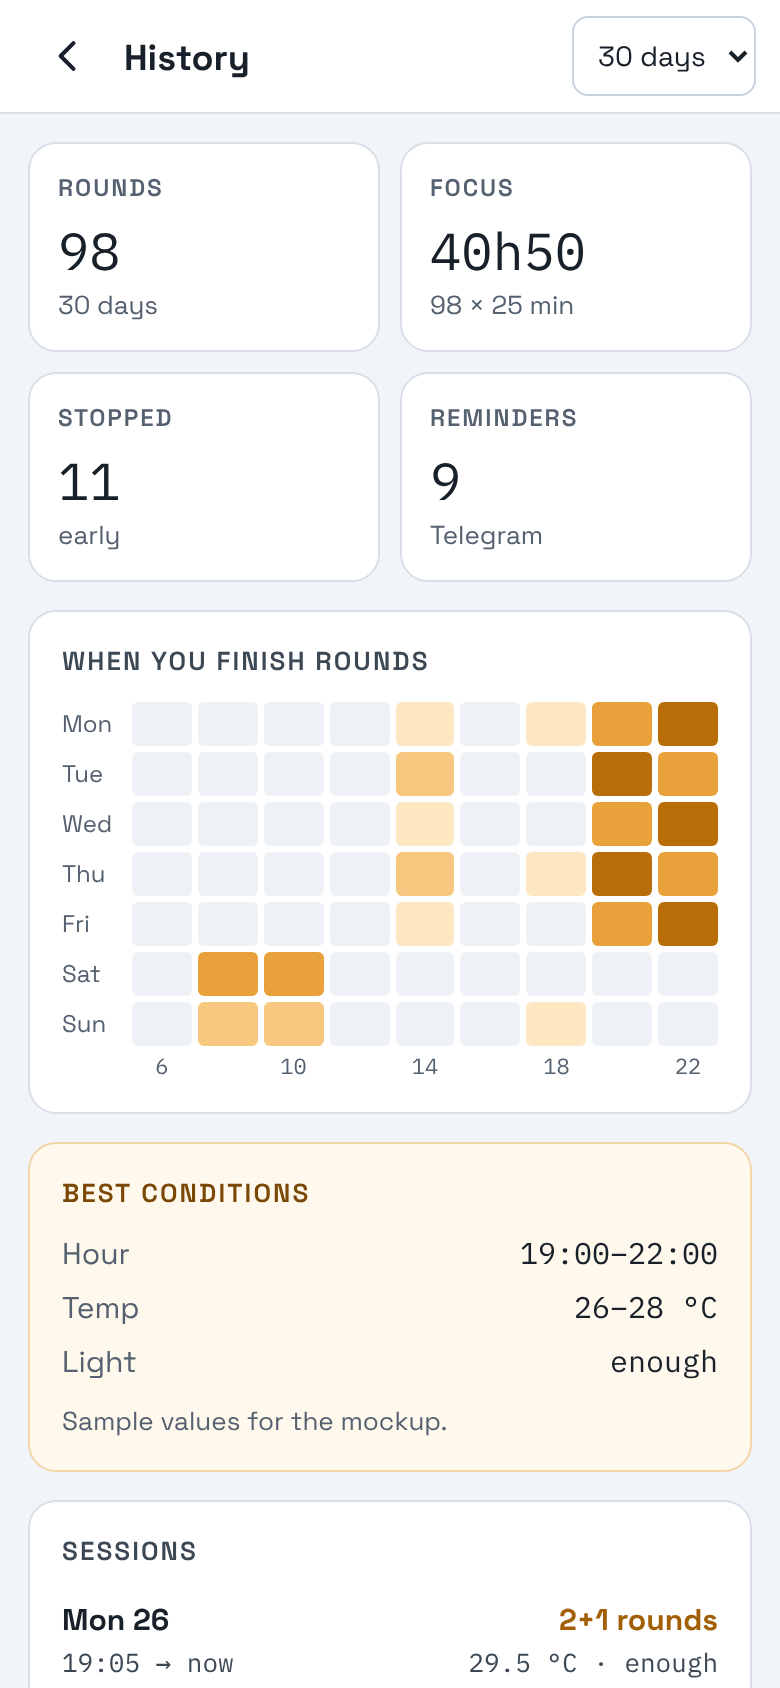
\includegraphics[width=\textwidth]{assets/wireframes/10-history-mobile.png}
    \caption{Lịch sử trên Mobile}
    \label{fig:history_mobile}
\end{subfigure}
\caption{Giao diện Thống kê và Lịch sử phiên học trên Desktop và Mobile}
\label{fig:history}
\end{figure}

\subsection{Màn hình Cài đặt hệ thống}
Cho phép người dùng tùy chỉnh các ngưỡng hoạt động (ngưỡng cảnh báo học quá lâu, ngưỡng thiếu sáng), cập nhật thông tin Telegram Chat ID và cấu hình tài khoản cá nhân.

\begin{figure}[htbp]
\centering
\begin{subfigure}[b]{0.62\textwidth}
    \centering
    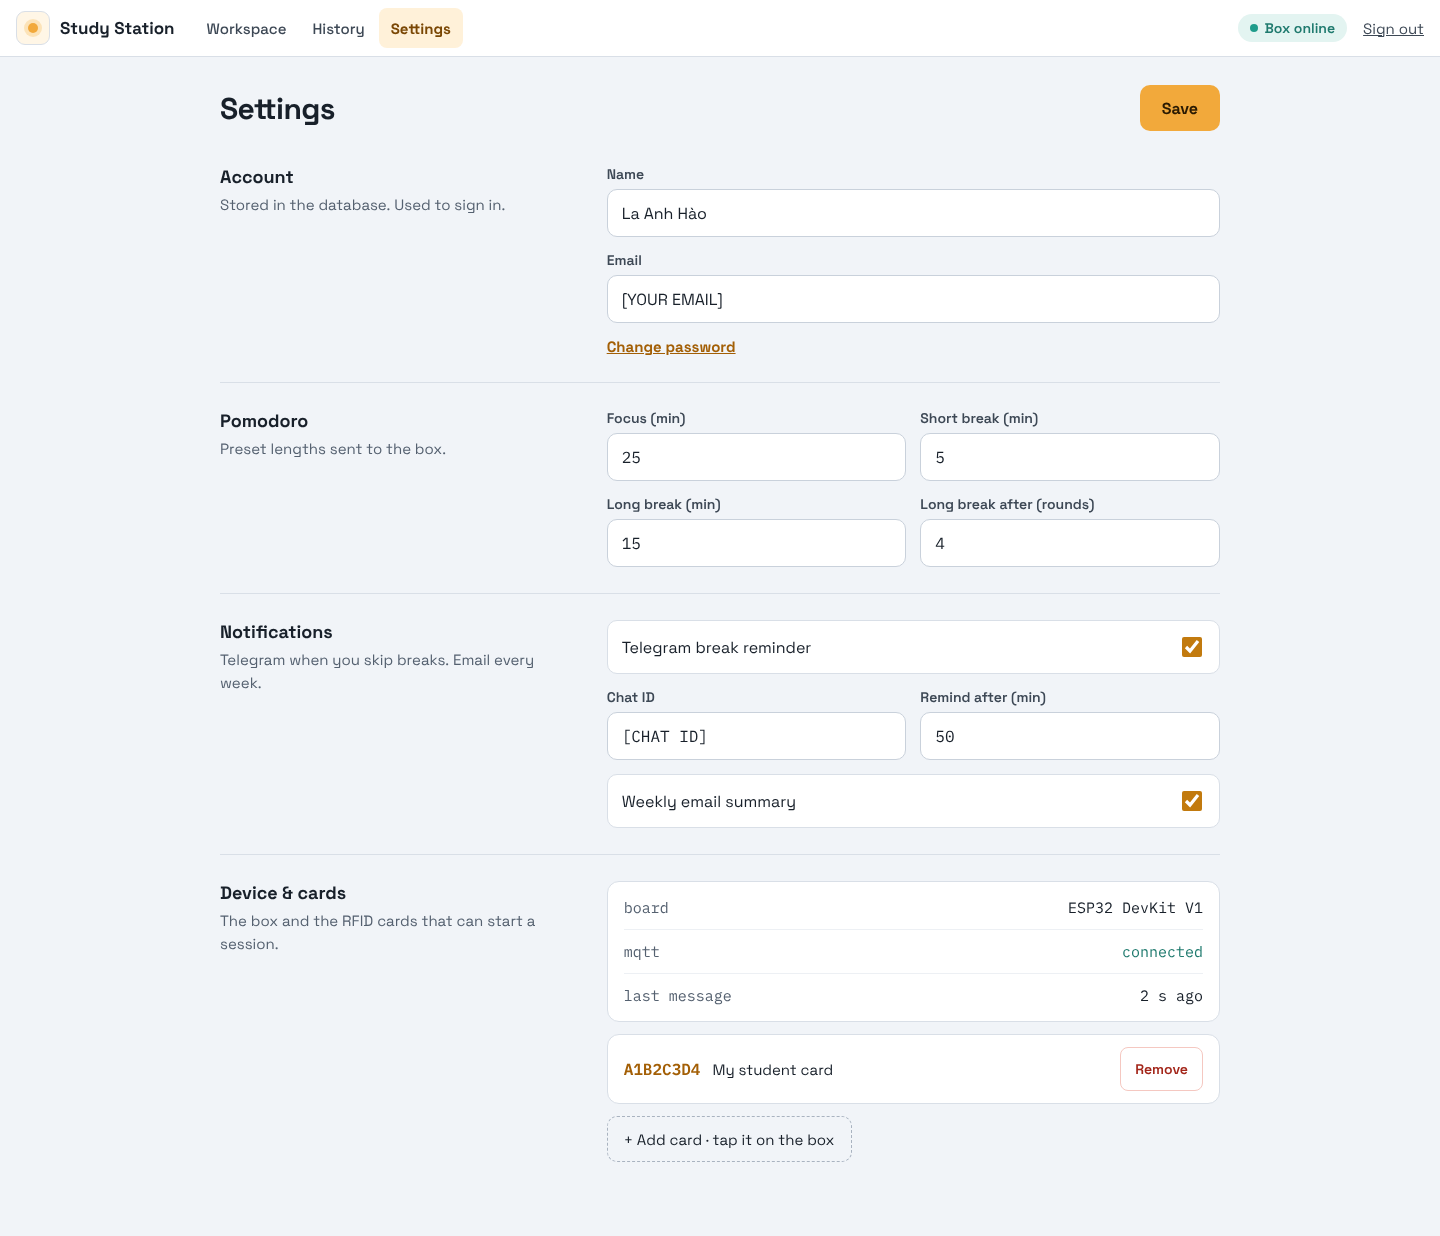
\includegraphics[width=\textwidth]{assets/wireframes/04-settings-desktop.png}
    \caption{Cài đặt hệ thống trên Desktop}
    \label{fig:settings_desktop}
\end{subfigure}
\hfill
\begin{subfigure}[b]{0.32\textwidth}
    \centering
    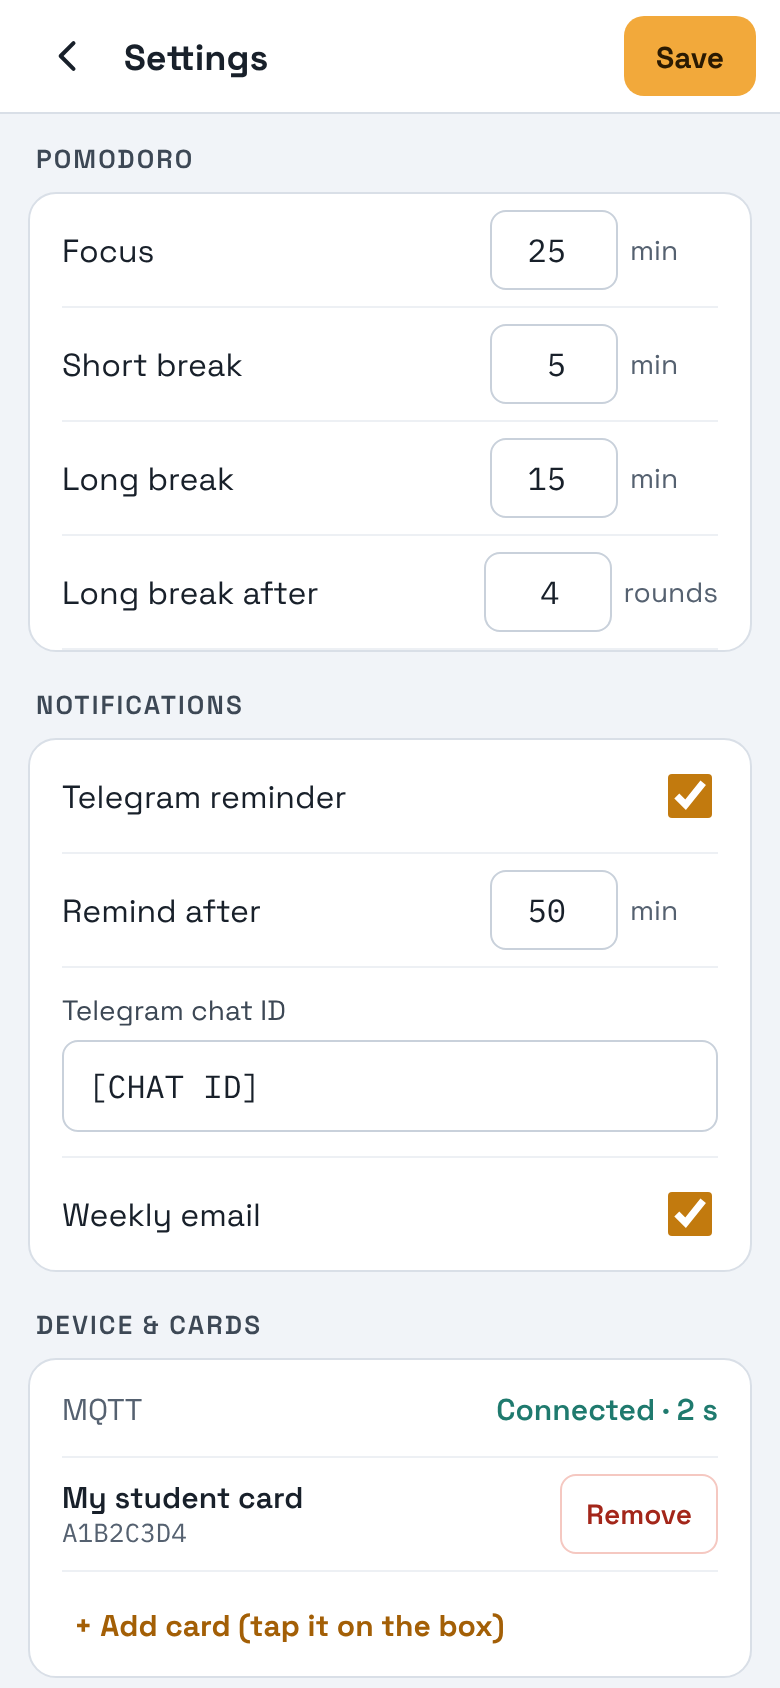
\includegraphics[width=\textwidth]{assets/wireframes/11-settings-mobile.png}
    \caption{Cài đặt trên Mobile}
    \label{fig:settings_mobile}
\end{subfigure}
\caption{Giao diện Cài đặt hệ thống và cấu hình thông số hoạt động}
\label{fig:settings}
\end{figure}
